\scanpage{140}
\unsure{1} sommet\\
1 face\\
2 arêtes\\
\unsure{4} repères, correspondent\\
aux rives des arêtes $a,b$

\deleted{$\sigma_0,\ \unsure{\sigma_1}\ \unsure{\hat a}$}

$\sigma_0=\sigma_2$ échangent $a^+,a^-$ et $b^+,b^-$\\
$\sigma_1$ échange \deleted{$\unsure{a^+\text{ et }a^-}$} $a^+$ et $b^+$, $a^-$ et $b^-$\\
$\sigma$ échange $a^+$ et $b^-$, $b^+$ et $a^-$

\[\underbrace{\sigma_1,\sigma},\underbrace{\sigma_2,\sigma_0}_{\substack{\Vert\\\sigma'}}\]
subdivision barycentrique

$\sigma_0=\sigma_2$ soit $\sigma'$, commute à $\sigma$\\
$\sigma_1=\sigma\sigma'$,\\
\deleted{$\unsure{\sigma=\sigma_1\sigma'}$}

\[\underbrace{\sigma\sigma'}_{\sigma_1},\underbrace{\sigma}_{\sigma},
\underbrace{\underbrace{\sigma'}_{\sigma_2},\underbrace{\sigma'}_{\sigma_0}}\]
\[\underbrace{\sigma\sigma'}_{\sigma'_0},\underbrace{\sigma'}_{\sigma'_1},\underbrace{\sigma}_{\sigma'_2}\]
\figure{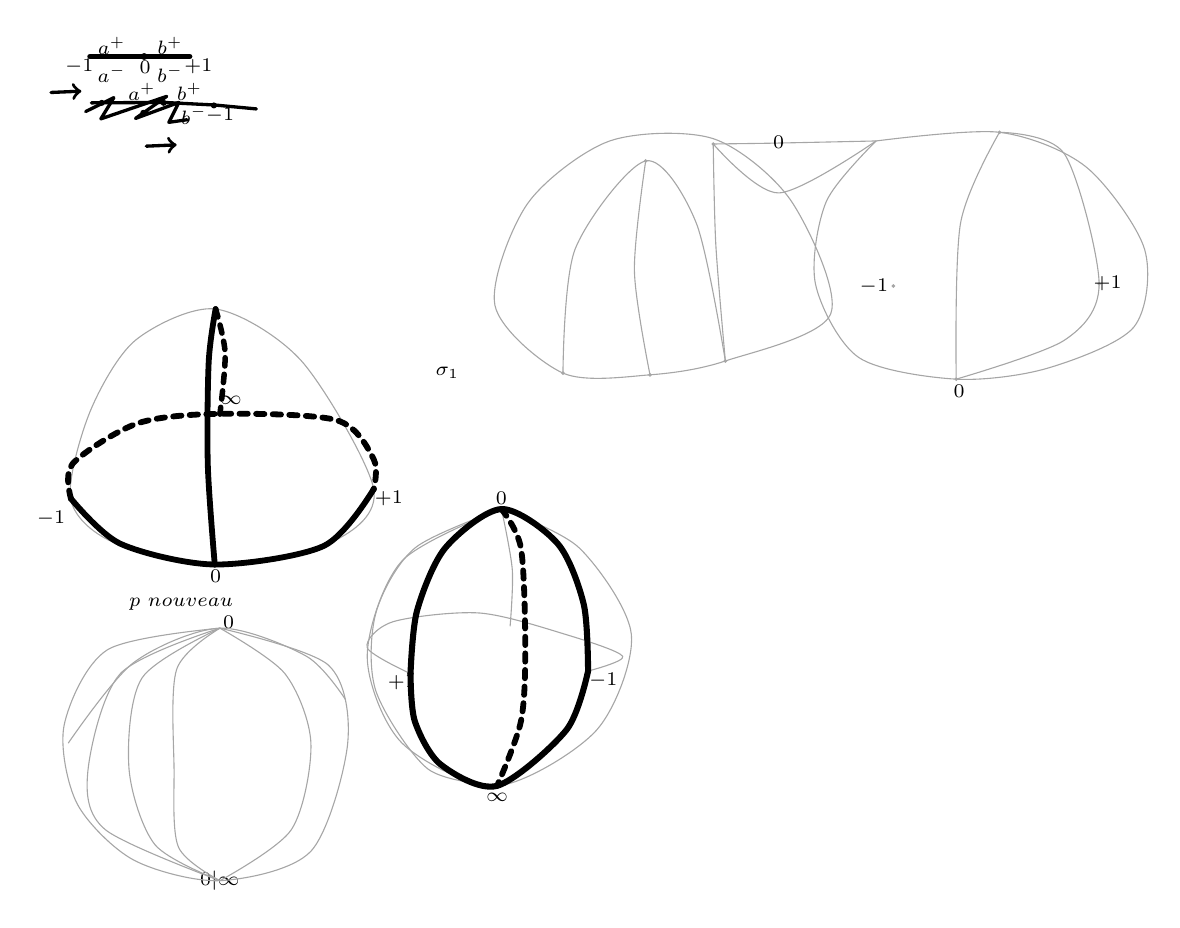
\begin{tikzpicture}[x=.55cm,y=-.55cm,line cap=round,line join=round,g/.style={olive!80!yellow,line width=1.7pt},r/.style={orange!80!brown,line width=1.8pt},w/.style={red!60!black,line width=1.5pt},b/.style={blue!60!black,line width=1.4pt},p/.style={gray!70,thin},k/.style={black,line width=1.2pt},every node/.style={font=\scriptsize}]
% Upper-left segments and overdrawn segment.
\draw[k,line width=2pt] (3.0,1.15)--(5.3,1.15);
\fill[k] (4.25,1.15) circle (.08);
\node at (2.75,1.37) {$-1$};
\node at (5.5,1.37) {$+1$};
\node at (4.27,1.4) {$0$};
\node at (3.5,.9) {$a^+$};
\node at (4.85,.9) {$b^+$};
\node at (3.5,1.55) {$a^-$};
\node at (4.85,1.55) {$b^-$};
\deleted{\begin{scope}
\draw[k] (3.03,2.22)--(4.7,2.21)--(5.88,2.27)--(6.84,2.36);
\draw[k] (2.9,2.42)--(3.55,2.1)--(3.25,2.59)--(4.77,2.07)--(4.05,2.58)--(5.05,2.21)--(4.82,2.67)--(5.24,2.61);
\fill[k] (3.27,2.22) circle (.07);
\fill[k] (4.7,2.22) circle (.07);
\fill[k] (4.23,2.45) circle (.07);
\fill[k] (5.86,2.28) circle (.07);
\node at (4.2,1.97) {$a^+$};
\node at (5.3,1.97) {$b^+$};
\node at (5.4,2.51) {$b^-$};
\node at (6,2.5) {$\unsure{-1}$};
\end{scope}}
\draw[k,->] (2.1,1.98)--(2.8,1.95);
\draw[k,->] (4.3,3.22)--(5.0,3.19);
% Upper pencil globes.
\draw[p] plot[smooth cycle] coordinates {(12.35,6.9) (13.1,4.55) (15.0,3.1) (17.4,3.05) (19.2,4.5) (20.1,7.1) (17.67,8.18) (15.93,8.5) (13.92,8.46)};
\draw[p] plot[smooth] coordinates {(13.92,8.46) (14.2,5.6) (15.83,3.56) (17.0,5.0) (17.67,8.18)};
\draw[p] plot[smooth] coordinates {(15.83,3.56) (15.57,6.1) (15.93,8.5)};
\draw[p] plot[smooth] coordinates {(17.39,3.17) (17.45,5.5) (17.67,8.18)};
\draw[p] plot[smooth] coordinates {(17.39,3.17) (18.8,3.15) (21.15,3.1)};
\draw[p] plot[smooth] coordinates {(17.39,3.17) (18.9,4.3) (21.15,3.1)};
\draw[p] plot[smooth] coordinates {(21.15,3.1) (20.0,4.5) (19.75,6.4) (20.75,8.1) (23.0,8.6) (25.1,8.35) (27.1,7.4) (27.35,5.6) (26.0,3.7) (24.0,2.9) (21.15,3.1)};
\draw[p] plot[smooth] coordinates {(24.0,2.9) (23.1,5.0) (23.0,8.6)};
\draw[p] plot[smooth] coordinates {(24.0,2.9) (25.5,3.4) (26.3,6.4) (25.5,7.7) (23.0,8.6)};
\fill[p] (13.92,8.46) circle (.045);
\fill[p] (15.83,3.56) circle (.045);
\fill[p] (15.93,8.5) circle (.045);
\fill[p] (17.39,3.17) circle (.045);
\fill[p] (17.67,8.18) circle (.045);
\fill[p] (21.55,6.45) circle (.045);
\fill[p] (24.0,2.9) circle (.045);
\fill[p] (26.3,6.4) circle (.045);
\fill[p] (23.0,8.6) circle (.045);
\node at (18.9,3.12) {$\unsure{0}$};
\node at (11.25,8.45) {$\sigma_1$};
\node at (21.1,6.45) {$-1$};
\node at (26.5,6.4) {$+1$};
\node at (23.07,8.88) {$0$};
% Large left ink ellipse with pencil construction.
\draw[p] plot[smooth cycle] coordinates {(2.55,11.35) (3.0,9.35) (4.05,7.7) (5.9,6.98) (7.9,8.2) (9.55,11.14) (8.6,12.35) (5.88,12.88) (3.5,12.35)};
\draw[k,line width=2.1pt] plot[smooth] coordinates {(2.56,11.36) (3.7,12.4) (5.88,12.88) (8.4,12.45) (9.55,11.14)};
\draw[k,line width=2.1pt,dashed] plot[smooth] coordinates {(2.56,11.36) (2.6,10.55) (4.1,9.62) (6.0,9.4) (8.7,9.55) (9.55,10.45) (9.55,11.14)};
\draw[k,line width=2.1pt] plot[smooth] coordinates {(5.9,6.98) (5.74,8.2) (5.72,10.6) (5.88,12.88)};
\draw[k,line width=2pt,dashed] plot[smooth] coordinates {(5.9,6.98) (6.12,8.0) (6.0,9.4)};
\fill[k] (2.56,11.36) circle (.07);
\fill[k] (9.55,11.14) circle (.07);
\fill[k] (5.88,12.88) circle (.07);
\fill[k] (6.0,9.4) circle (.07);
\node at (2.1,11.82) {$-1$};
\node at (9.9,11.35) {$+1$};
\node at (5.9,13.15) {$0$};
\node at (6.25,9.1) {$\infty$};
% Faint lower-left globe.
\node at (5.1,13.8) {$\unsure{p\ \text{nouveau}}$};
\node at (6.2,14.22) {$0$};
\node at (6.0,20.18) {$\unsure{0|\infty}$};
\draw[p] plot[smooth] coordinates {(6.0,14.35) (3.4,14.85) (2.4,16.6) (2.7,18.4) (4.0,19.7) (6.0,20.18) (8.1,19.5) (8.95,17.0) (8.5,15.2) (6.0,14.35)};
\draw[p] plot[smooth] coordinates {(6.0,14.35) (5.0,15.3) (4.94,17.6) (5.04,19.4) (6.0,20.18)};
\draw[p] plot[smooth] coordinates {(6.0,14.35) (4.2,15.5) (3.9,17.6) (4.5,19.35) (6.0,20.18)};
\draw[p] plot[smooth] coordinates {(6.0,14.35) (3.7,15.4) (2.95,17.65) (3.35,19.0) (6.0,20.18)};
\draw[p] plot[smooth] coordinates {(6.0,14.35) (7.5,15.4) (8.1,17.0) (7.65,19.0) (6.0,20.18)};
\draw[p] plot[smooth] coordinates {(2.5,17.0) (4.0,15.15) (6.0,14.35) (8.0,15.0) (8.9,16.0)};
% Lower central oval with dashed meridian and faint surrounding constructions.
\draw[p] plot[smooth] coordinates {(12.5,11.6) (10.2,12.8) (9.4,15.0) (10.2,17.0) (12.4,17.99) (14.7,16.7) (15.5,14.5) (14.3,12.5) (12.5,11.6)};
\draw[p] plot[smooth] coordinates {(12.5,11.6) (10.5,12.5) (9.6,14.0) (9.6,15.8) (10.8,17.6) (12.4,17.99)};
\draw[p] plot[smooth] coordinates {(10.4,15.4) (9.4,14.8) (10.0,14.2) (12.0,14.0) (14.0,14.5) (15.3,15.0) (14.5,15.34)};
\draw[p] plot[smooth] coordinates {(12.5,11.6) (12.75,13.0) (12.7,14.3)};
\draw[k,line width=2.2pt] plot[smooth] coordinates {(10.4,15.4) (10.55,13.95) (11.2,12.5) (12.5,11.6) (13.8,12.4) (14.4,13.8) (14.5,15.34)};
\draw[k,line width=2.2pt] plot[smooth] coordinates {(14.5,15.34) (14.0,16.7) (12.4,17.99) (11.1,17.5) (10.5,16.5) (10.4,15.4)};
\draw[k,line width=2.1pt,dashed] plot[smooth] coordinates {(12.5,11.6) (12.95,12.5) (13.05,14.8) (12.95,16.5) (12.4,17.99)};
\fill[k] (10.4,15.4) circle (.065);
\fill[k] (14.5,15.34) circle (.065);
\fill[k] (12.4,17.99) circle (.065);
\node at (12.5,11.35) {$0$};
\node at (12.4,18.25) {$\infty$};
\node at (10.2,15.6) {$\unsure{+1}$};
\node at (14.85,15.55) {$-1$};
\end{tikzpicture}}
\margin{\mspage{139}}
